

\section{Introduction and Module Walkthrough}

\begin{frame}{About Myself: Jan Suchanek}
    \mytext{
    \begin{itemize}
        \item Diplom-Volkswirt (MA Economics)
        \item MBL (Master of Business Law)
        \item born in Hamburg, based in Berlin
        \item English, German (native), French, Spanish        
        \item Project Manager: Energy Networking Projects
        \item Teaching Project Management
        \item Teaching Microeconomics
        \item ...and this class
    \end{itemize}
    }
\end{frame}

\begin{frame}{About Yourself}
    \mytext{
        \begin{itemize}
            \item ISGM students
            \item Incoming Students?
            \item favourite market / country?
        \end{itemize}
    }
\end{frame}

\begin{frame}{Schedule}
\mytext{
    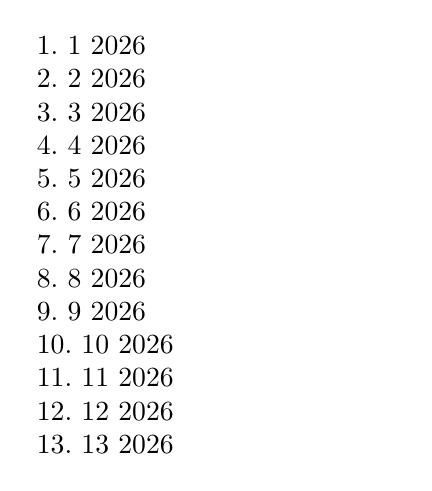
\begin{tikzpicture}
        \node at (0,0) {
        \parbox{30ex}%
        {
        \foreach \i in {1,...,13}
            {\i.~\mysession{\i} \the\year\par}
        }
        };
    \end{tikzpicture}

    Dates and announcements are on 
    \href{https://aulis.hs-bremen.de/goto.php/crs/2216491}{AULUS (link)}
}
\mycomment{
    AULIS serves as central platform for our communication. Whenever possible, use it. In particular, do not send me files per email (ever!), and do not send me emails from a private, non-HSB server. Such emails will be ignored.

    The course language is English. Communication in languages other than English will also be ignored.

    Materials will be uploaded: presentation, and white cover scripts.

    If you have special needs, please let me know.
}
    
\end{frame}


\begin{frame}{Schedule}
    \mytext{
        \begin{itemize}
            \item April - July: Lectures
            \item Students choose an example market
            \item \textbf{May 19th: Student Presentations}
            \begin{itemize}
                \item 9:00 - 17:00 hrs
                \item a raw material / commodity market
                \item a country dominated by that market                
            \end{itemize}
            \item \textbf{June 30th: Student Demos}
            \begin{itemize}
                \item 9:00 - 17:00 hrs
                \item an international organisation and
                \item a company active in that market
            \end{itemize}
            \item \textbf{End July: written exam}
        \end{itemize}

        \medskip    
    }
    \mycomment{
    Your presentation is typically 10-20 minutes long. Students present the topic using slide shows. Please do not show video / animations, unless you practice thoroughly. 

    Your demo is free speach on the subject, using available web resources that you can share with the audience live. In particular, you should demo how we can use the information present at the websites of the organisations to access valuable data.

    Tipp: create one (!) slide with the links (bookmarks) to the pages (and sub-pages) that you want to show.

    The nature of the written exam is yet to be decided and declared.

    % Your summary letter is a short letter to your lecturer expressing what you have learned, what questions remain, what your main take-aways are, and what could be improved in this module in the future.
    
    }
\end{frame}


\begin{frame}{Market, Country, Organisation, Company}
    \showmytikz[1]{../shared/tikz/tikz-market-organisations.tex}
    \mycomment{
        You are holding two double presentations, or better: one double presentation and one double demo.

        The connecting link is the commodity (or service) X on which you focus. This should be a raw material or merchandise, not a branded or customised product.

    }
\end{frame}

\begin{frame}{Market, Country, Organisation, Company}
    \showmytikz[1,2]{../shared/tikz/tikz-market-organisations.tex}
    \mycomment{
        The country can be an individual state, or a close-knit group of states (e.g. EU). 
        
    }
\end{frame}
\begin{frame}{Market, Country, Organisation, Company}
    \showmytikz[1,2,3]{../shared/tikz/tikz-market-organisations.tex}
    \mycomment{
        The company could be purely trading, but also mining, refining, or processing X. Choose an MNE (multi-national enterprise).

        The organisation could be a private body - typically, an industry association - or an intergovernmental body.

    }
\end{frame}

\begin{frame}{Students Presentation of the Market for a Product}
    \mytext{
    Analyse and present the market of a particular good:
    \begin{enumerate}
        \item delimitation of the market
        \item price, volumes, market places        
        \item elasticities, substitutes
        \item connected markets / use
        \item buyers, sellers, regulators
        \item trends (price, volumens, technology)
        \item future prices, volatility, insurance
        \item global connections, trade routes
        \item externalities    
    \end{enumerate}
    }
    \mycomment{
    You may treat some of these aspects jointly unless your group is large enough to cover these all.

    We will of course cover the meaning of these terms in the lecture.
    }
\end{frame}


\begin{frame}{Students Presentation of the Country}
    \mycomment{    
    The exercise is to study a particular country, which plays a somehow significant role in the chosen market. This can be as importer, but more likely will be that of an exporter. 
    
    We would like to understand the role of the market for the country and the role of the country for the market, the most important actors, the development of the country and the market, the relation between the economy of the country and the development of the market.    
    }
    \mytext{
    Tell us about the country of your choice:
    \begin{itemize}
        \item Terrain, climate, traffic etc: show a map
        \item Demographics: population, age
        \item Income distribution, GDP, GDP per capita
        \item Growth, currency, size of informal sector
        \item Industry, agriculture
        \item Balance of Payments
        \item Relevance of the market for country
        \item Main players, areas, ports
        \item Perspectives
    \end{itemize}
    }
\end{frame}


\begin{frame}{Technical Requirements: Presentation}
    \mytext{
    \begin{itemize}
        % \item students grouped by lecturer
        \item work in groups
        \item every student presents
        \item[] one aspect on one slide
        \item create consistency in design and content
        \item upload \textbf{as .pdf} on the day
        \item also bring .pdf on a USB stick
        \item[] (or on phone with USB-HDMI adapter)
        \item grading is 50\% individual  and 50\% group work quality.
    \end{itemize}
    }
    \mycomment{
    Course language is English. Communication in any other language will be ignored. 

    Abstain from sending obscure proprietary or unnecessarily bloated formats. NEVER send attachments. Upload only .pdf.

    For email enquiries, use your HSB email only: requests from obscure email addresses will be treated as spam.

    }
\end{frame}

\begin{frame}{Technical Requirements: Demo of Company and Organsation}
    \mytext{
    \begin{itemize}
        \item same groups (some regrouping possible)
        \item talk using projector to show sources
        \item show how to find important information on the company and organisation websites
        \item describe the work of company and organisation
        \item mention other players / competitors
        \item provide an outlook
        \item \textbf{NO SLIDES}
    \end{itemize}
    }
    \mycomment{
    The idea here is that you talk about the company and the international organisation, presenting them to class.

    You can demo live how to use their websites to find important information about them - their publications, data bases they offer, reports etc.

    You demonstrate your ability to critically use these sources of information. Dig deeper than the landing pages. You can also show other pages with relevant information.
    }
\end{frame}



\begin{frame}{Grading}
    \mytext{
    The portfolio exam parts are weighted:
    
    40\% M1 Presentation I+II \\
    40\% M2 Presentation (demo) III+IV \\
    20\% M3 written exam  
    }
    \mycomment{
    The first two of these parts are presentations. At M1, you are to present a market and a country. At M2, you are to talk about a company and an international organisation, using projection and screen share to demonstrate your knowledge and show us what there is to know about these institutions. M3 is going to be a small exam / test / quizz.
    }
\end{frame}


\begin{frame}{Grading}
    \mytable{
       \begin{tabular}{lllll}
        \toprule
        Latin & \multicolumn{2}{l}{Traditional} & Modern & English  \\
        \midrule \midrule
            summa cum laude & 1 & \multirow{2}{*}{sehr gut} & 1,0 & \multirow{2}{*}{very good}  \\
            magna cum laude & 1- &   & 1,3 &    \\
            \midrule
            \multirow{3}{*}{bene} & 2+ & \multirow{3}{*}{gut} & 1,7 &  \multirow{3}{*}{good} \\
             & 2 &   & 2,0 &   \\
             & 2- &   & 2,3 &   \\
             \midrule
            \multirow{3}{*}{rite} & 3+ & \multirow{3}{*}{befriedigend} & 2,7 & \multirow{3}{*}{satisfying} \\
             & 3 & & 3,0 &  \\
             & 3- &  & 3,3 &  \\
             \midrule
            \multirow{2}{*}{sufficienter} & 4+ & \multirow{2}{*}{ausreichend} & 3,7 & \multirow{2}{*}{sufficient} \\
             & 4 &  & 4,0 &  \\
            \midrule
            \midrule
            insufficienter & 5 & ungenügend & 5,0 & insufficient (fail)\\
            \midrule
            sub omne canone & 6 & Leistungsverweigerung & 5,0 & no-show \\
            \bottomrule
        \end{tabular}
    }        
\end{frame}

\begin{frame}{Etiquette}
    \mytext{
    \begin{itemize}
        \item Classes start s.t. (sin tempore, punctually)
        \item 5 minutes small talk / sound check
        \item cameras on!
        \item address with first name
        \item I use Aulis forum for announcements
        \item You use Aulis forum to announce your choices
        \item no sending of files!
    \end{itemize}
    }
\end{frame}

% \section{Markets of Interest}

\begin{frame}{Raw Materials, Commodities, Merchandise}
    \mycomment{
        Examples for raw materials are iron ore, and crude oil; once refined, they become commodities such as steel, and petrol; from which we produce manufactured goods, which when traded are called merchandise.

        Note that services can also be traded, and for other traded objects other vocabulary may apply. For example, you can trade bonds, or you can trade derivatives.

        So in a sense raw materials are a sub-class of commodities, and commodities are a sub-class of  merchandise. This is, however, a conventional distinction, not a legal one, and usage may vary.



    }
    \showmytikz[1]{../shared/tikz/tikz-raw-commodities}
\end{frame}
\begin{frame}{Raw Materials, Commodities, Merchandise}
    \mycomment{
        Along the value chain, various means of production are needed. In principle these are capital and labour. These are in parts themselves tradable. 

        Most commodities require more than one raw material as input: fertiliser is used to grow corn, energy needed to process iron ore and create steel. And when it comes to merchandise, each packaging and distribution step adds a large amount to the price.        

        Typically, the different stages of production are not happening at the same place. So there is trade involved between most stages. 
    }
    \showmytikz[1,2]{../shared/tikz/tikz-raw-commodities}
\end{frame}
\begin{frame}{Raw Materials, Commodities, Merchandise}
    \mycomment{
        Trade is not instantaneous, and it is not just magically happening. It is intrinsically linked to logistics. It includes transport over a distance, and often also over trade barriers such as customs borders or through choke points. 
    
        It also requires financial flows in the opposite direction.

        Since trade does not happen without buyers, the sales costs are typically added. This includes the fees for wholesalers, grossists and retailers, which typically constitute more than half of the consumer end price of merchandise due to costs for transport, marketing, shop keeping, advertisement, sales etc.
    }
    \showmytikz[1,2,3]{../shared/tikz/tikz-raw-commodities}
\end{frame}


\begin{frame}{Some Interesting Global Markets/Goods}
    \mycomment{
        You have time until next week to decide / propose your own example market.

        You may also propose your own working team.

        Students who have not voiced their own preference and team will receive assignment.           
    }   
    \mytext{
    Hard commodities:
    \mylonglist{
            \begin{itemize}
                \item non-iron industrial metals
                \begin{itemize}
                    \item cobalt
                    \item tungsten
                    \item conflict minerals: tin, tantalum, wolfram, gold
                \end{itemize}
                \item iron ore, steel
                \item other minerals
                \begin{itemize}
                    \item phosphate
                    \item cement, sand, gipsum
                \end{itemize}
            \end{itemize}
     }
    }
\end{frame}


\begin{frame}{Some Interesting Global Markets/Goods}
    \mytext{
    \mylonglist{
  
  Soft commodities:
        \begin{itemize}
            \item nutmeg / spices
            \item latex, logs / lumber
            \item cotton, wool
            \item garments / fabrics
            \item plastic / base chemicals
        \end{itemize}

    Carbohydrates:
        \begin{itemize}
            \item crude oil
            \item liquified natural gas (LNG)
            \item petrol
            \item chemicals, pharmaceuticals
            \item base plastics
        \end{itemize}
    }
    }
\end{frame}


% \begin{frame}{Some Interesting Global Markets/Goods}
%     \mytext{    
%     \mylonglist{
    
%         \begin{itemize}
%             \item dry edibles, fruit juice, vegetable oil
%             \item fast moving consumer goods FMCGs
%             \item grains (wheat, rice, corn, soy)
%             \item precision gear wheels
%             \item crude oil, LNG, petrol
%             \item household waste
%             \item certificates of origin (CoOs), ETS \ce{CO2} emission rights
%             \item military equipment, dual use goods
%             \item machinery: packaging, harvesting, industrial robots
%             \item rare earths, other non-iron metals
%         \end{itemize}
%     }
%     }
% \end{frame}

% \begin{frame}{Some Interesting Global Markets/Goods}
%     \mytext{    
%     \mylonglist{
    
%         \begin{itemize}
%             \item government bonds  (of Japan, US...)
%             \item currency, precious metals, gold, diamonds
%             \item insurances, financial services
%             \item microchips (particular class)
%             \item scrap metal
%             \item shipping containers
%             \item cars, lorries, airplanes
%             \item pumps and pipes
%             \item rail equipment
%             \item barbed wire
%         \end{itemize}
%     }
%     }
% \end{frame}


% \section{Market Characteristics}

\begin{frame}{Market  Characteristics}
    \mycomment{
    You should apply what you have learned in Microeconomics when describing the market. This applies to the delimitation and other core characteristica. Of course, you need not comment on every possible quality, but only point out remarkable characteristics.
    }
    \mytext{
        \begin{itemize}
            \item spacial delimitation (`where')
            \item temporal deliminination (`when')
            \item by characteristics
            \begin{itemize}
                \item substitutiability: buyer side
                \item substitutiability: seller side
            \end{itemize}
            \item market access / barriers to entry
            \item information restraints
        \end{itemize}    
        }
\end{frame}

\begin{frame}{Market Characteristics}
    \mycomment{
    Apart from general characteristics, please provide core data and figures. How large is this market? Where is it heading? Who dominates it?
    }
    \mytext{
        \begin{itemize}
            \item market history
            \item adjacent markets
            \item players: buyers, sellers
            \item regulators, regulations
            \item physical properties
            \item factor markets
            \item market volumes
            \item market segments
            \item elasticities
        \end{itemize}
    }
\end{frame}

% \section{Types of Goods and Markets}

\begin{frame}{Different Types of Goods}
\mytable{
    \begin{tabular}{lll|l}
        \toprule
                    & price $\nearrow$     & income $\nearrow$    & example \\
        \midrule
                    
        \textbf{normal}      & \textbf{demand $\searrow$}  & \textbf{demand $\nearrow$}    & soap  \\
        inferior    & demand $\searrow$  & demand $\searrow$  & cheap noodles \\
        Veblen      & demand $\nearrow$    & demand $\nearrow$   & luxury watches \\
        Giffen      & demand $\nearrow$    & demand $\searrow$  & rice \\
        \bottomrule
    \end{tabular}
}
        
\end{frame}

\begin{frame}{Substitutes and Complements}
    \mytext{
    \begin{itemize}
        \item \textbf{substitute goods:} price and demand negatively correlated
        \item[] e.g. margarine and butter
        \item \textbf{complementary goods:} price and demand positively correlated
        \item[] e.g. printers and cartridges
    \end{itemize}
    }
\end{frame}



\begin{frame}{Types of Tradables}
    \mytext{
    \begin{itemize}
        \item goods vs. services
        \item immaterial goods, intellectual property
        \item rights and patents (not: innovations)
        \item means of production, land, labour
        \item perishables, durables
        \item intermediate goods
        \item investment goods, machines
        \item resources, raw materials
    \end{itemize}
    }
\end{frame}
\begin{frame}{Physical Qualities}
    \mytext{
    \begin{itemize}
        \item break bulk cargo
        \item general cargo
        \item LCL less than car load
        \item logistics and trade
        \item information and organisation, data
        \item intangible assets, marketing, attention
    \end{itemize}
    }
\end{frame}



% \section{Some Interesting Visualisation Tools}

\begin{frame}{Harvard: Atlas of Economic Complexity}
    \mycomment{This tool is a very good visualisation of trade patterns and of the Balance of Payments of various countries.

    Please browse this tool. You will surely find inspiration for your tasks ahead.
    }
    \showmybitmap[https://atlas.hks.harvard.edu/]{../shared/bitmaps/ATLAS-HKS-HARVARD-EDU.png}
\end{frame}

\begin{frame}{IMF: IMF Data Mapper}
    \showmybitmap[https://www.imf.org/external/datamapper/]{../shared/bitmaps/IMF-DATAMAPPER.png}
\end{frame}

\begin{frame}{World Bank: WITS}
    \showmybitmap[https://wits.worldbank.org/]{../shared/bitmaps/WITS.png}
\end{frame}

\begin{frame}{Bertelsmann: GEDVIZ}
    \showmybitmap[https://viz.ged-project.de/]{../shared/bitmaps/GEDVIZ.png}
\end{frame}

\begin{frame}{MIT: OEC}
    \showmybitmap[https://oec.world/en]{../shared/bitmaps/OEC.png}
\end{frame}

